\documentclass[a4paper,12pt]{article}
\usepackage[brazil, english]{babel}
\usepackage[utf8]{inputenc}
\usepackage[T1]{fontenc}
\usepackage{geometry}
\usepackage{setspace}
\usepackage{titlesec}
\usepackage{hyperref}
\usepackage{graphicx}
\usepackage{caption}
\usepackage{subcaption}
\usepackage{fancyhdr}
\setlength{\headheight}{15pt}
\addtolength{\topmargin}{-2.5pt}
\usepackage{xcolor}
\usepackage{amsmath, amssymb, bm}
\usepackage{mathtools}
\usepackage{cancel}
\usepackage{tikz}
\usepackage{newunicodechar}
\usepackage{ragged2e}
\usepackage{setspace}
\usepackage{tikz-3dplot} % Necessário para coordenadas 3D
\usetikzlibrary{intersections}
\usepackage{siunitx}
\usetikzlibrary{3d, arrows.meta}

\usepackage{color}
\definecolor{myblue}{rgb}{.8, .8, 1}

\usepackage{amsmath}
\usepackage{empheq}

\newlength\mytemplen
\newsavebox\mytempbox

\makeatletter
\newcommand\mybluebox{%
    \@ifnextchar[%]
       {\@mybluebox}%
       {\@mybluebox[0pt]}}

\def\@mybluebox[#1]{%
    \@ifnextchar[%]
       {\@@mybluebox[#1]}%
       {\@@mybluebox[#1][0pt]}}

\def\@@mybluebox[#1][#2]#3{
    \sbox\mytempbox{#3}%
    \mytemplen\ht\mytempbox
    \advance\mytemplen #1\relax
    \ht\mytempbox\mytemplen
    \mytemplen\dp\mytempbox
    \advance\mytemplen #2\relax
    \dp\mytempbox\mytemplen
    \colorbox{myblue}{\hspace{1em}\usebox{\mytempbox}\hspace{1em}}}
\makeatother

\usepackage[most]{tcolorbox}

\newtcbox{\mymath}[1][]{%
    nobeforeafter, math upper, tcbox raise base,
    enhanced, colframe=blue!30!black,
    colback=blue!30, boxrule=1pt,
    #1}

\tcbset{
    highlight math style={
        enhanced,
        colframe=red!60!black,
        colback=yellow!50,
        arc=4pt,
        boxrule=1pt,
        drop fuzzy shadow
    }
    }

\usepackage{physics}
\usepackage{pgfplots}
\pgfplotsset{compat=1.17}

\linespread{1.5}

\definecolor{ao(english)}{rgb}{0.0, 0.5, 0.0}
\definecolor{byzantium}{rgb}{0.44, 0.16, 0.39}
\newunicodechar{∘}{\circ}

%%%%%%%%%%%%%%%%%%%%%%%%%%%%%%%%%%%%%%%%%%%%%%%%%%
% These are some new commands that may be useful 
% for paper writing in general. If other new commands
% are needed for your specific paper, please feel 
% free to add here. 
%
% The currently available commands are organized in: 
% 1) Systems
% 2) Quantities
% 3) Energies and units
% 4) particle species
% 5) Colors package
% 6) hyperlink
%%%%%%%%%%%%%%%%%%%%%%%%%%%%%%%%%%%%%%%%%%%%%%%%%%

\usepackage{amsmath}
\usepackage{amssymb}
\usepackage{upgreek}
\usepackage{multirow}
\usepackage{setspace}% http://ctan.org/pkg/setspace
\usepackage{fancyhdr}
\usepackage{datetime}

% 1) SYSTEMS
\newcommand{\btc}               {\textbf{BTC}}
\newcommand{\btcspace}          {\textbf{BTC} }
\newcommand{\pow}               {\textbf{PoW}}

% 4) definition to references, biblatex and hyperlink
\usepackage[backend=bibtex, 
style=nature,  %style reference.
sorting=none,
firstinits=true %first name abbreviate
]{biblatex}

\usepackage{hyperref}
\hypersetup{
    colorlinks=true, %set "true" if you want colored links
    linktoc=all,     %set to "all" if you want both sections and subsections linked
    linkcolor=blue,  %choose some color if you want links to stand out
    citecolor= blue, % color of \cite{} in the text.
    urlcolor  = blue, % color of the link for the paper in references.
}

% 5) Tikz and figures
\usepackage{epsfig}
\usepackage{lmodern}
\usepackage{mathtools}
\usepackage[utf8]{luainputenc}
\usepackage{xspace}
\usepackage{tikz}
\usepackage{pgfplots}
\pgfplotsset{compat=newest}

\usetikzlibrary{positioning}
\usepackage{subcaption}

% 6) colors:
\usepackage{xcolor}
\definecolor{ao(english)}{rgb}{0.0, 0.5, 0.0} % dark green

% 7) Add lines numbers
%\usepackage{lineno}

% add pdf file to thesis:
\usepackage{pdfpages}

\hypersetup{
    colorlinks=true,% make the links colored
    linkcolor=blue
}

\usepackage{setspace}
\addbibresource{bibliography.bib}

\newcommand{\printingbibliography}{%

    \pagestyle{myheadings}
    \markright{}
    \sloppy
    \printbibliography[heading=bibintoc, % add to table of contents
                   title=Refer\^encias % Chapter name
                  ]
    \fussy%
}
\PassOptionsToPackage{table}{xcolor}

\pagestyle{fancy}
\fancyhf{}
\renewcommand{\headrulewidth}{0pt}
\fancyhead[R]{\thepage}

\geometry{a4paper,top=30mm,bottom=20mm,left=30mm,right=20mm}

\titleformat*{\section}{\bfseries\large}
\titleformat*{\subsection}{\bfseries\normalsize}

\title{ \textbf{\large Eletromagnetismo I }}
\author{Andr\'e V. Silva}
\date{\today}

\begin{document}

\noindent\rule{\linewidth}{0.8pt}\\
\begin{center}
    \textbf{UNIVERSIDADE FEDERAL DO RIO DE JANEIRO}\\
    \textbf{INSTITUTO DE FÍSICA}\\
    \textbf{\textcolor{blue}{Segunda lista complementar de Eletromagnetismo 1}}\\
    \textbf{Maio de 2025}\\
    \vspace{0.5cm}
    Prof. João Torres de Mello Neto\\
    Monitor: Pedro Khan
\end{center}
\noindent\rule{\linewidth}{0.8pt}\\
\maketitle


\noindent\rule{\linewidth}{0.4pt}\\

\justifying

\begin{flushleft}
\textbf{\textcolor{blue}{\Large Problema 1}}\\

Dois planos condutores aterrados ao longo dos eixos \(x\) e \(y\) se 
interceptam na origem, conforme mostrado na figura. Uma carga \(q\) 
é colocada a uma distância \(b\) acima do eixo \(x\) e a uma distância 
\(a\) à direita do eixo \(y\). Determine a força sobre a carga.\\

\noindent
\textbf{Sugestão:} as cargas imagens devem fazer com que as condições de 
contorno sejam mantidas nos dois planos simultaneamente.

\vspace{0.5cm}

\begin{center}
\begin{tikzpicture}[scale=1.2]
  % Eixos
  \draw[->, thick] (0,0) -- (4,0) node[below right] {\(x\)};
  \draw[->, thick] (0,0) -- (0,4) node[above left] {\(y\)};

  % Carga q
  \filldraw[red] (3,3) circle (2pt) node[right] {\(q\)};
  
  % Linhas tracejadas para indicar a e b
  \draw[dashed] (3,0) -- (3,3);
  \draw[dashed] (0,3) -- (3,3);

  % Setas para indicar a e b
  \draw[<->] (0,-0.5) -- (3,-0.5) node[midway, below] {\(a\)};
  \draw[<->] (-0.5,0) -- (-0.5,3) node[midway, left] {\(b\)};
\end{tikzpicture}
\end{center}

\textcolor{red}{\textbf{Solução:}}\\

Como os planos condutores estão aterrados, o potencial ao longo dos eixos \(x = 0\) e \(y = 0\) deve ser nulo. Para satisfazer essa condição, usaremos o \textbf{método das cargas imagem}.

A carga real \(q\) está localizada no ponto \((a, b)\), com \(a > 0\) e \(b > 0\), no primeiro quadrante. Para que o potencial seja nulo nos eixos coordenados, inserimos três cargas imagem:

\begin{itemize}
  \item Uma carga imagem \(-q\) em \((-a, b)\), que anula o potencial no plano \(x = 0\),
  \item Uma carga imagem \(-q\) em \((a, -b)\), que anula o potencial no plano \(y = 0\),
  \item Uma carga imagem \(+q\) em \((-a, -b)\), que garante simultaneamente que o potencial seja zero nos dois planos.
\end{itemize}

\bigskip

\begin{center}
\begin{tikzpicture}[scale=1.0]
  % Eixos
  \draw[->, thick] (-4,0) -- (4,0) node[below right] {\(x\)};
  \draw[->, thick] (0,-4) -- (0,4) node[above left] {\(y\)};

  % Carga real q
  \filldraw[red] (3,3) circle (2pt) node[above right] {\(q\)};

  % Carga imagem 1: (-q) em (-3,3)
  \filldraw[blue] (-3,3) circle (2pt) node[above left] {\(-q\)};

  % Carga imagem 2: (-q) em (3,-3)
  \filldraw[blue] (3,-3) circle (2pt) node[below right] {\(-q\)};

  % Carga imagem 3: (+q) em (-3,-3)
  \filldraw[blue] (-3,-3) circle (2pt) node[below left] {\(q\)};

  % Linhas tracejadas para indicar a e b
  \draw[dashed] (3,0) -- (3,3);
  \draw[dashed] (0,3) -- (3,3);

  % Setas para indicar a e b
  \draw[<->] (0,-0.8) -- (3,-0.8) node[midway, below] {\(a\)};
  \draw[<->] (-0.8,0) -- (-0.8,3) node[midway, left] {\(b\)};
\end{tikzpicture}
\end{center}

\subsection*{Cálculo da força}

A força total sobre a carga real \(q\) é a soma das forças de Coulomb exercidas pelas cargas imagem.

\subsubsection*{Força devido a \(-q\) em \((-a, b)\):}
\begin{equation}
\vec{F}_1 = \frac{1}{4\pi\varepsilon_0} \cdot \frac{q(-q)}{(2a)^2} \hat{i} = -\frac{q^2}{16\pi\varepsilon_0 a^2} \hat{i}
\end{equation}

\subsubsection*{Força devido a \(-q\) em \((a, -b)\):}
\begin{equation}
\vec{F}_2 = \frac{1}{4\pi\varepsilon_0} \cdot \frac{q(-q)}{(2b)^2} \hat{j} = -\frac{q^2}{16\pi\varepsilon_0 b^2} \hat{j}
\end{equation}

\subsubsection*{Força devido a \(+q\) em \((-a, -b)\):}

A distância até a carga real é \(2\sqrt{a^2 + b^2}\). O vetor deslocamento é \((2a, 2b)\), portanto:

\begin{equation}
\vec{F}_3 = \frac{1}{4\pi\varepsilon_0} \cdot \frac{q^2}{(2\sqrt{a^2 + b^2})^2} \cdot \frac{(2a, 2b)}{2\sqrt{a^2 + b^2}} 
= \frac{q^2}{16\pi\varepsilon_0 (a^2 + b^2)^{3/2}} (a\hat{i} + b\hat{j})
\end{equation}

\subsection*{Resultado final}

Somando os três termos:

\begin{equation}
\vec{F} = \vec{F}_1 + \vec{F}_2 + \vec{F}_3
\end{equation}

\begin{equation}
\boxed{
\vec{F} = \frac{q^2}{16\pi \varepsilon_0} \left[
\left( -\frac{1}{a^2} + \frac{a}{(a^2 + b^2)^{3/2}} \right) \hat{i} +
\left( -\frac{1}{b^2} + \frac{b}{(a^2 + b^2)^{3/2}} \right) \hat{j}
\right]
}
\end{equation}

\end{flushleft}


\begin{flushleft}
\textbf{\textcolor{blue}{\Large Problema 2}}\\

Uma distribuição de carga elétrica produz o campo elétrico
\begin{equation}
\mathbf{E} = c \left( 1 - e^{-\alpha r} \right) \frac{\hat{\mathbf{r}}}{r^2}
\end{equation}
onde \(c\) e \(\alpha\) são constantes. Encontre a carga total dentro do raio \(r = \frac{1}{\alpha}\).

\textcolor{red}{\textbf{Solução:}}\\

Utilizaremos o \textbf{teorema de Gauss}, que relaciona o fluxo do campo elétrico com a carga total no interior de uma superfície fechada:

\begin{equation}
\oint_{\text{superfície}} \mathbf{E} \cdot d\mathbf{A} = \frac{Q_{\text{int}}}{\varepsilon_0}
\end{equation}

Como o campo é radial e depende apenas de \(r\), escolhemos uma superfície gaussiana esférica de raio \(r = \frac{1}{\alpha}\). O campo elétrico sobre essa superfície tem módulo:
\begin{equation}
|\mathbf{E}(r)| = c \left( 1 - e^{-\alpha r} \right) \frac{1}{r^2}
\end{equation}

O vetor de área é \(d\mathbf{A} = \hat{\mathbf{r}}\, r^2 \sin\theta\, d\theta\, d\phi\), portanto:
\begin{equation}
\Phi_E = \oint \mathbf{E} \cdot d\mathbf{A} = |\mathbf{E}(r)| \cdot 4\pi r^2
\end{equation}

Substituindo:
\begin{align}
\Phi_E &= c \left(1 - e^{-\alpha r} \right) \cdot \frac{1}{r^2} \cdot 4\pi r^2 \\
&= 4\pi c \left(1 - e^{-\alpha r} \right)
\end{align}

Aplicando o teorema de Gauss:
\begin{equation}
Q_{\text{int}} = \varepsilon_0 \Phi_E = 4\pi \varepsilon_0 c \left(1 - e^{-\alpha r} \right)
\end{equation}

Finalmente, substituímos \(r = \frac{1}{\alpha}\):
\begin{equation}
Q = 4\pi \varepsilon_0 c \left(1 - e^{-1} \right)
\end{equation}

\section*{Resposta final}

\begin{equation}
\boxed{Q = 4\pi \varepsilon_0 c \left(1 - \frac{1}{e} \right)}
\end{equation}

\end{flushleft}

\begin{flushleft}
\textbf{\textcolor{blue}{\Large Problema 3}}\\

Uma haste fina e não condutora de comprimento \( l \) carrega uma carga 
\( Q \) uniformemente distribuída e está orientada conforme mostrado na figura:

\begin{center}
\begin{tikzpicture}[scale=1.5]
  % Eixos coordenados
  \draw[->, thick] (0,0) -- (1.8,0) node[below] {\(y\)};
  \draw[->, thick] (0,0) -- (0,2.2) node[above] {\(z\)};
  \draw[->, thick] (0,0) -- (-1.5,-1.0) node[left] {\(x\)};

  % Haste carregada (em vermelho)
  \draw[very thick, red] (0,-1) -- (0,1);
  \node[left] at (0,0) {\(Q\)};

  % Parte não carregada dos eixos z
  \draw[thick] (0,-1.5) -- (0,-1); % abaixo da haste
  \draw[thick] (0,1) -- (0,1.5);   % acima da haste

  % Marcas para +l/2 e -l/2
  \node[right] at (0,1) {\(\frac{l}{2}\)};
  \node[right] at (0,-1) {\(-\frac{l}{2}\)};
\end{tikzpicture}
\end{center}

\begin{enumerate}
    \item[(a)] Determine o potencial \( V \) devido à haste carregada para qualquer 
    ponto sobre o eixo \( z \), com \( z > l/2 \).

    \item[(b)] Encontre \( V(r, \theta, \varphi) \) para todos os pontos com \( |\mathbf{r}| > l/2 \), 
    onde \( r, \theta, \varphi \) são as coordenadas esféricas usuais.
\end{enumerate}

\textbf{Sugestão para a parte b:} A solução geral da equação de Laplace em coordenadas esféricas 
com simetria azimutal é dada por
\begin{equation}
V(r, \theta) = \sum_{l=0}^{\infty} \left( A_l r^l + \frac{B_l}{r^{l+1}} \right) P_l(\cos\theta),
\qquad \text{Griffiths, 3.65},
\end{equation}

Os \colorbox{green!15}{coeficientes são determinados a partir das condições de contorno de cada problema.}

\textcolor{red}{\textbf{Solução:}}\\

\subsection*{(a) Potencial sobre o eixo \( z \) com \( z > \frac{l}{2} \)}

A densidade linear de carga da haste é
\begin{equation}
\lambda = \frac{Q}{l}
\end{equation}

O potencial eletrostático gerado por uma linha de carga no ponto \( z \) (com \( z > l/2 \)) é dado por:
\begin{equation}
V(z) = \frac{1}{4\pi\varepsilon_0} \int_{-l/2}^{l/2} \frac{\lambda \, dz'}{|z - z'|}
\end{equation}

Como \( z > z' \) em todo o intervalo, podemos retirar o módulo:
\begin{equation}
V(z) = \frac{\lambda}{4\pi\varepsilon_0} \int_{-l/2}^{l/2} \frac{dz'}{z - z'} = \frac{\lambda}{4\pi\varepsilon_0} \left[ \ln(z - z') \right]_{z' = -l/2}^{z' = l/2}
\end{equation}

\begin{equation}
V(z) = \frac{\lambda}{4\pi\varepsilon_0} \ln\left( \frac{z + l/2}{z - l/2} \right)
\end{equation}

\noindent\textbf{Resposta da parte (a):}
\begin{equation}
\boxed{V(z) = \frac{\lambda}{4\pi\varepsilon_0} \ln\left( \frac{z + l/2}{z - l/2} \right)}
\quad \text{para } z > \frac{l}{2}
\end{equation}

\subsection*{(b) Potencial em coordenadas esféricas para \( r > \frac{l}{2} \)}

\colorbox{yellow}{A solução geral da equação de Laplace com simetria azimutal é}:
\begin{equation}
\boxed{
V(r, \theta) = \sum_{l=0}^{\infty} \left( A_l r^l + \frac{B_l}{r^{l+1}} \right) P_l(\cos\theta)
}
\end{equation}

Como estamos \colorbox{blue!15}{fora da distribuição de cargas, não há termo crescente (\( A_l = 0 \))}, então:

\begin{equation}
\boxed{
V(r, \theta) = \sum_{l=0}^{\infty} \frac{B_l}{r^{l+1}} P_l(\cos\theta)
}
\end{equation}

Os coeficientes \( B_l \) são dados por:
\begin{equation}
B_l = \frac{1}{\varepsilon_0 (2l+1)} \int \rho(\vec{r}') \, (r')^l \, P_l(\cos\theta') \, d\tau'
\end{equation}

Como \colorbox{green!25}{a carga está ao longo do eixo \( z \)}, temos:

\[
r' = |\bm{r}'| = |z'|, \qquad \cos\theta' = \frac{z'}{|z'|}.
\]

Portanto, \colorbox{green!25}{o polinômio de Legendre avaliado no ângulo $\theta'$} é:

\[
P_l(\cos\theta') = P_l\left( \frac{z'}{|z'|} \right) =
\begin{cases}
\boxed{P_l(1) = 1}, & \text{se } z' > 0, \\
P_l(-1) = (-1)^l, & \text{se } z' < 0.
\end{cases}
\]

\begin{equation}
\rho(\vec{r'}) = \lambda \, \delta(x') \delta(y') \Rightarrow dq = \lambda \, dz'
\quad \text{e} \quad \cos\theta' = \frac{z'}{|z'|}
\end{equation}

Então:
\begin{equation}
\boxed{
B_l = \frac{\lambda}{\varepsilon_0(2l+1)} \int_{-l/2}^{l/2} (z')^l P_l(1)\, dz'}
\end{equation}

\begin{equation}
\boxed{
B_l = \frac{\lambda}{\varepsilon_0(2l+1)} \int_{-l/2}^{l/2} (z')^l \, dz'
} \hspace{0.3cm} \checkmark
\end{equation}

\textbf{Paridade:}
\begin{itemize}
\item \colorbox{red!15}{Para \( l \) ímpar: integral de função ímpar \(\Rightarrow 0\)}
\item \colorbox{green!15}{Para \( l \) par: integral de função par \(\Rightarrow 2 \int_0^{l/2} z'^l \, dz'\)}
\end{itemize}

\vspace{0.3cm}
\noindent
\colorbox{green!15}{\textbf{Termo monopolar (\( l = 0 \)):}}
\begin{equation}
B_0 = \frac{\lambda}{\varepsilon_0} \int_{-l/2}^{l/2} dz' = \frac{\lambda l}{\varepsilon_0} = \frac{Q}{\varepsilon_0}
\end{equation}

\begin{equation}
V_0(r) = \frac{1}{4\pi\varepsilon_0} \cdot \frac{Q}{r}
\end{equation}

\vspace{0.3cm}
\noindent
\colorbox{blue!15}{\textbf{Termo quadrupolar (\( l = 2 \)):}}

\begin{equation}
B_2 = \frac{\lambda}{5\varepsilon_0} \int_{-l/2}^{l/2} (z')^2 \, dz' = \frac{\lambda}{5\varepsilon_0} \cdot \frac{l^3}{12}
= \frac{\lambda l^3}{60\varepsilon_0}
\end{equation}

\begin{equation}
V_2(r, \theta) = \frac{1}{4\pi\varepsilon_0} \cdot \frac{\lambda l^3}{60 r^3} \cdot \left( \frac{3\cos^2\theta - 1}{2} \right)
\end{equation}

\vspace{0.3cm}
\noindent
\colorbox{red!15}{\textbf{Termo octopolo (\( l = 4 \)):}}

\begin{equation}
B_4 = \frac{\lambda}{9\varepsilon_0} \int_{-l/2}^{l/2} (z')^4 \, dz' = \frac{\lambda}{9\varepsilon_0} \cdot \frac{l^5}{80}
= \frac{\lambda l^5}{720\varepsilon_0}
\end{equation}

\begin{equation}
V_2(r, \theta) = \frac{1}{4\pi\varepsilon_0} \cdot \frac{\lambda l^5}{720 r^5} \cdot \left( \frac{35\cos^4\theta - 30\cos^2\theta + 3}{8} \right)
\end{equation}


\vspace{0.3cm}
\noindent
\textbf{Resposta da parte (b):}

\begin{equation}
\boxed{
V(r, \theta) \approx \frac{1}{4\pi\varepsilon_0} \left[
\textcolor{green}{\frac{Q}{r}} +
\textcolor{blue}{\frac{\lambda l^3}{60 r^3} \left( \frac{3\cos^2\theta - 1}{2} \right)}
+ \textcolor{red}{\frac{\lambda l^5}{720 r^5} \cdot \left( \frac{35\cos^4\theta - 30\cos^2\theta + 3}{8} \right)}
+ \cdots
\right]
,\quad r > \frac{l}{2}
}
\end{equation}

% Solution Here
\end{flushleft}

\begin{flushleft}
\textbf{\textcolor{blue}{\Large Problema 4}}\\

Considere uma esfera de raio \( a \) contendo uma densidade de carga uniforme \( \rho \) no 
seu interior, e sem carga no exterior. Deseja-se determinar o potencial eletrostático \( V(r) \) 
e o campo elétrico \( \mathbf{E}(r) \) em todo o espaço, \colorbox{red!20}{assumindo que \( V \rightarrow 0 \) 
quando \( r \rightarrow \infty \)}. 

Determine o campo elétrico dentro e fora da esfera. Resolva a equação de Poisson para dentro 
e fora da esfera.

\textbf{Obs:} esse problema foi resolvido muitas vezes desde Física 3 por meio da lei 
de Gauss na formulação integral.

\textcolor{red}{\textbf{Solução:}}\\

% Solution Here
\section*{1. Campo Elétrico via Lei de Gauss}

Pela simetria esférica, o campo elétrico é radial, ou seja, \( \mathbf{E}(r) = E(r)\, \hat{r} \). Utilizamos a Lei de Gauss:

\begin{equation}
\boxed{\oint \mathbf{E} \cdot d\mathbf{A} = \frac{Q_{\text{int}}}{\varepsilon_0}}
\end{equation}

\subsection*{\colorbox{green!15}{Para \( r < a \) (interior da esfera):}}

\begin{equation}
Q_{\text{int}} = \rho \cdot \frac{4}{3}\pi r^3
\Rightarrow E(r) \cdot 4\pi r^2 = \frac{\rho \cdot \frac{4}{3}\pi r^3}{\varepsilon_0}
\Rightarrow \boxed{E(r) = \frac{\rho r}{3\varepsilon_0}}
\end{equation}

\subsection*{\colorbox{red!15}{Para \( r > a \) (exterior da esfera):}}

\begin{equation}
Q = \rho \cdot \frac{4}{3} \pi a^3
\Rightarrow E(r) \cdot 4\pi r^2 = \frac{Q}{\varepsilon_0}
\Rightarrow \boxed{E(r) = \frac{1}{4\pi\varepsilon_0} \cdot \frac{Q}{r^2}
= \frac{\rho a^3}{3\varepsilon_0 r^2}}
\end{equation}

\begin{figure}[h]
\centering
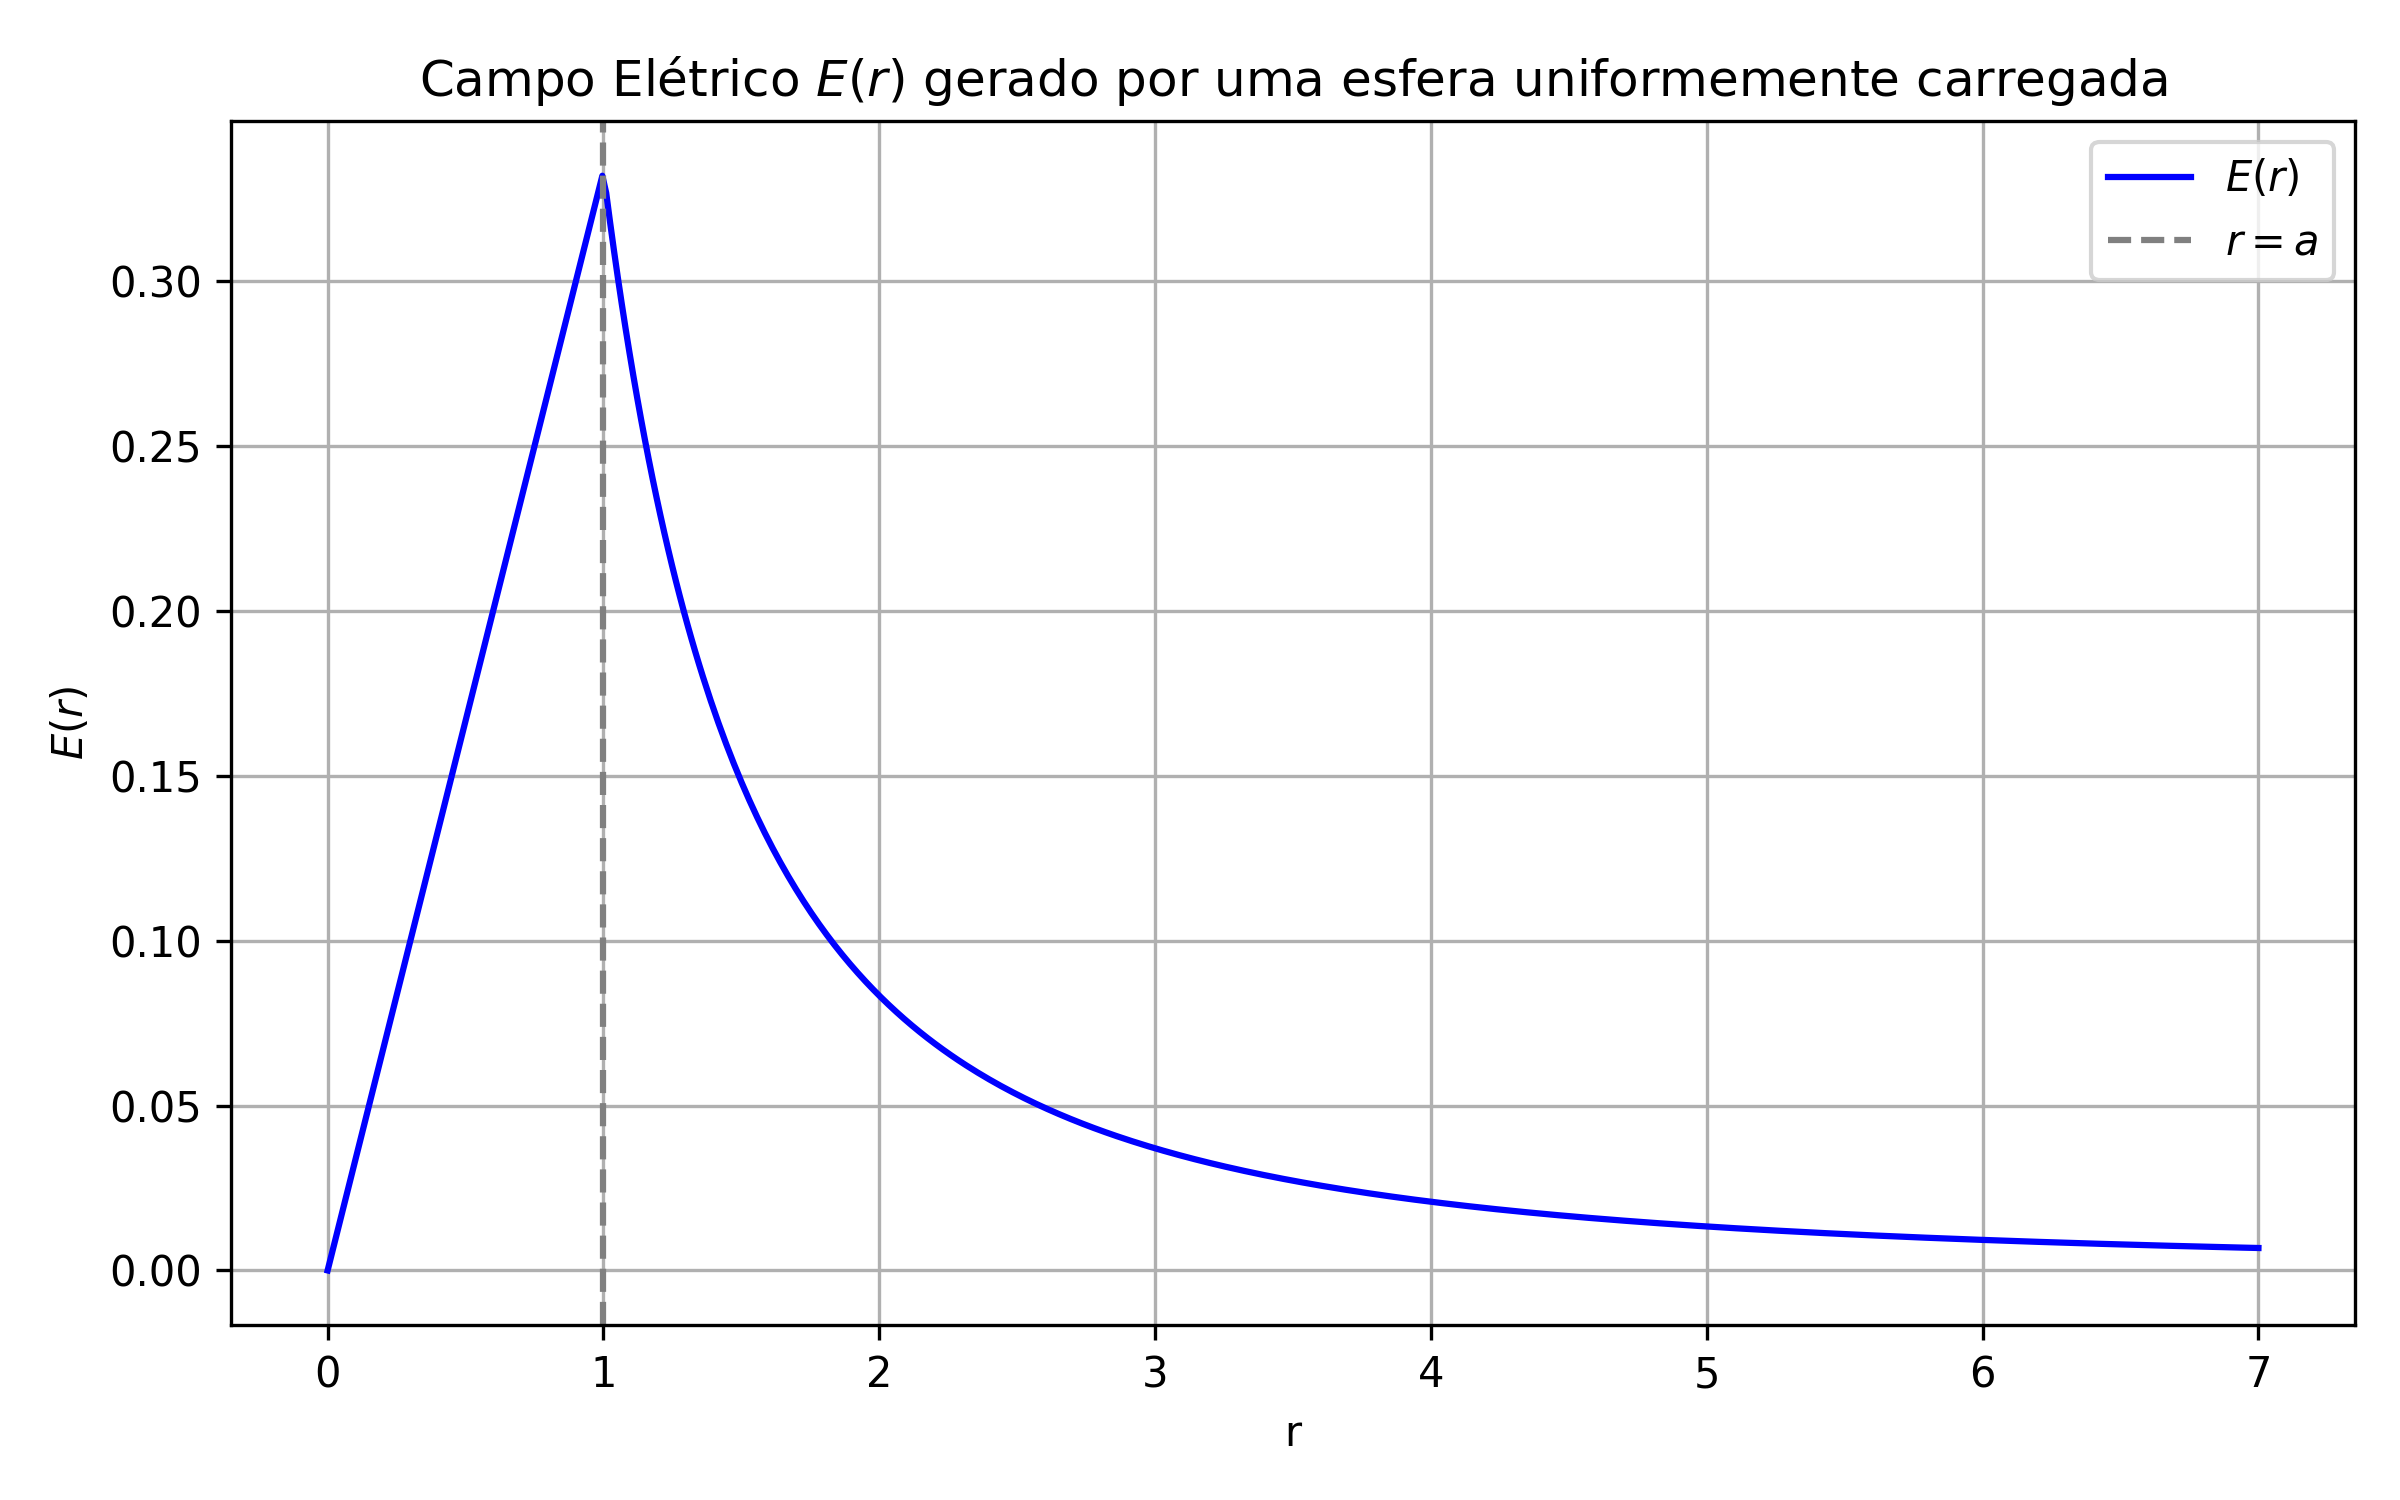
\includegraphics[width=0.9\textwidth]{plots/campo_eletrico_esfera.png} % Substitua por seu nome de arquivo
\caption{Campo elétrico dentro e fora da esfera.}
\end{figure}

\newpage
\section*{2. Potencial Elétrico via Equação de Poisson}

A \colorbox{green!15}{equação de Poisson para simetria esférica é:}

\begin{equation}
\frac{1}{r^2} \dv{r} \left( r^2 \dv{V}{r} \right) = -\frac{\rho(r)}{\varepsilon_0}
\end{equation}

\subsection*{\colorbox{green!15}{Para \( r < a \) (com \( \rho = \text{constante} \))}}

\begin{equation}
\frac{1}{r^2} \dv{r} \left( r^2 \dv{V}{r} \right) = -\frac{\rho}{\varepsilon_0}
\Rightarrow \dv{r} \left( r^2 \dv{V}{r} \right) = -\frac{\rho r^2}{\varepsilon_0}
\end{equation}

Integrando:

\begin{equation}
r^2 \dv{V}{r} = -\frac{\rho}{\varepsilon_0} \cdot \frac{r^3}{3} + C_1
\Rightarrow \dv{V}{r} = -\frac{\rho r}{3\varepsilon_0} + \frac{C_1}{r^2}
\end{equation}

Impondo "regularidade" significa que a solução (neste caso, 
o potencial \( V(r) \) deve ser finita e bem-comportada em todos os pontos 
do domínio físico, incluindo no centro da esfera \( r=0) \), temos \( C_1 = 0 \). Integrando novamente:

\begin{equation}
V(r) = -\frac{\rho}{6\varepsilon_0} r^2 + C_2
\end{equation}

\subsection*{\colorbox{red!15}{Para \( r > a \) (região sem carga)}}

\begin{equation}
\frac{1}{r^2} \dv{r} \left( r^2 \dv{V}{r} \right) = 0
\Rightarrow \dv{r} \left( r^2 \dv{V}{r} \right) = 0
\Rightarrow r^2 \dv{V}{r} = C_3
\Rightarrow \dv{V}{r} = \frac{C_3}{r^2}
\Rightarrow V(r) = -\frac{C_3}{r} + C_4
\end{equation}

\section*{3. Condições de Contorno}

\begin{itemize}
    \item \colorbox{green!15}{Continuidade do potencial em \( r = a \)}:
    \begin{equation}
    V_{\text{int}}(a) = V_{\text{ext}}(a)
    \end{equation}
    \item \colorbox{green!15}{Continuidade da derivada do potencial (campo elétrico) em \( r = a \)}:
    \begin{equation}
    \left. \dv{V}{r} \right|_{r=a^-} = \left. \dv{V}{r} \right|_{r=a^+}
    \end{equation}
    \item \colorbox{green!15}{Condição no infinito: \( V(r) \rightarrow 0 \Rightarrow C_4 = 0 \)}
\end{itemize}

Derivadas:

\begin{equation}
\left. \dv{V}{r} \right|_{r=a^-} = -\frac{\rho a}{3\varepsilon_0}, \quad
\left. \dv{V}{r} \right|_{r=a^+} = \frac{C_3}{a^2}
\Rightarrow \boxed{C_3 = -\frac{\rho a^3}{3\varepsilon_0}}
\end{equation}

Potencial contínuo em \( r = a \):

\begin{equation}
-\frac{\rho}{6\varepsilon_0} a^2 + C_2 = \frac{\rho a^2}{3\varepsilon_0}
\Rightarrow \boxed{C_2 = \frac{\rho a^2}{2\varepsilon_0}}
\end{equation}

\section*{4. Resultados Finais}

\subsection*{Campo Elétrico}

\begin{equation}
\mathbf{E}(r) = 
\begin{cases}
\displaystyle \frac{\rho r}{3\varepsilon_0}\, \hat{r}, & r < a \\
\\
\displaystyle \frac{\rho a^3}{3\varepsilon_0 r^2}\, \hat{r}, & r > a
\end{cases}
\end{equation}

\subsection*{Potencial Elétrico}

\begin{equation}
V(r) = 
\begin{cases}
\displaystyle -\frac{\rho}{6\varepsilon_0} r^2 + \frac{\rho a^2}{2\varepsilon_0}, & r < a \\
\\
\displaystyle \frac{\rho a^3}{3\varepsilon_0 r}, & r > a
\end{cases}
\end{equation}
\end{flushleft}

\begin{flushleft}
\textbf{\textcolor{blue}{\Large Problema 5}}\\

Considere um tubo retangular de dimensões \( 0 \leq x \leq b \) e \( 0 \leq y \leq a \), infinito na direção \( z \).  
As fronteiras em \( x = 0 \), \( x = b \) e \( y = a \) estão mantidas a potencial nulo (\( V = 0 \)), enquanto  
a fronteira em \( y = 0 \) está mantida a um potencial constante \( V_0 \).  
Determinar o potencial eletrostático \( V(x, y) \) dentro do tubo.

\textcolor{red}{\textbf{Solução:}}\\

% Solution Here

Consideramos um tubo retangular definido por \( 0 \leq x \leq b \), \( 0 \leq y \leq a \), infinito na direção \( z \). O potencial eletrostático \( V(x, y) \) satisfaz a equação de Laplace bidimensional:

\begin{equation}
\frac{\partial^2 V}{\partial x^2} + \frac{\partial^2 V}{\partial y^2} = 0
\end{equation}

com as seguintes condições de contorno:

\begin{align*}
V(x, a) &= 0, \\
V(0, y) &= 0, \\
V(b, y) &= 0, \\
V(x, 0) &= V_0.
\end{align*}

Utilizando o \colorbox{yellow!25}{método de separação de variáveis}, assumimos uma solução do tipo:

\begin{equation}
V(x, y) = X(x)Y(y)
\end{equation}

Substituindo na equação de Laplace e separando variáveis, obtemos:

\begin{align*}
X''(x) + \lambda X(x) &= 0, \\
Y''(y) - \lambda Y(y) &= 0,
\end{align*}

com as soluções para \( X(x) \) que satisfazem \( X(0) = X(b) = 0 \):

\begin{equation}
X_n(x) = \sin\left( \frac{n\pi x}{b} \right), \quad \lambda_n = \left( \frac{n\pi}{b} \right)^2, \quad n = 1, 2, 3, \ldots
\end{equation}

A solução correspondente para \( Y(y) \), que satisfaz \( Y(a) = 0 \), é:

\begin{equation}
Y_n(y) = \sinh\left( \frac{n\pi (a - y)}{b} \right)
\end{equation}

Assim, a solução geral do potencial é:

\begin{equation}
\boxed{
V(x, y) = \sum_{n=1}^{\infty} C_n \sin\left( \frac{n\pi x}{b} \right) \sinh\left( \frac{n\pi (a - y)}{b} \right)}
\end{equation}

Impondo a condição \( V(x, 0) = V_0 \), obtemos a série de Fourier da função constante \( V_0 \):

\begin{equation}
V_0 = \sum_{n=1}^{\infty} C_n \sin\left( \frac{n\pi x}{b} \right) \sinh\left( \frac{n\pi a}{b} \right)
\end{equation}

Multiplicando ambos os lados por \( \sin\left( \frac{m\pi x}{b} \right) \) e integrando de \( 0 \) a \( b \), obtemos:

\begin{equation}
C_n = \frac{2}{b \sinh\left( \frac{n\pi a}{b} \right)} \int_0^b V_0 \sin\left( \frac{n\pi x}{b} \right) dx = \frac{4V_0}{n\pi \sinh\left( \frac{n\pi a}{b} \right)} \quad \text{para } n \text{ ímpar}
\end{equation}

Portanto, a solução final para o potencial dentro do tubo é:

\begin{equation}
\boxed{
V(x, y) = \sum_{\substack{n=1 \\ n\ \text{ímpar}}}^{\infty} \frac{4V_0}{n\pi \sinh\left( \frac{n\pi a}{b} \right)} \sin\left( \frac{n\pi x}{b} \right) \sinh\left( \frac{n\pi (a - y)}{b} \right)
}
\end{equation}
\end{flushleft}

\begin{flushleft}
\textbf{\textcolor{blue}{\Large Problema 6}}\\

Em um dispositivo unidimensional, a densidade volumétrica de carga é dada por
\begin{equation}
\rho_v(x) = \rho_0 \frac{x}{a}
\end{equation}

\noindent
Sabendo que o campo elétrico \( E = 0 \) em \( x = 0 \) e o potencial \( V = 0 \) em \( x = a \), 
determinar as expressões para \( V(x) \) e \( \mathbf{E}(x) \).

\textcolor{red}{\textbf{Solução:}}\\

% Solution Here

Dada a densidade volumétrica de carga:

\begin{equation}
\rho_v(x) = \rho_0 \frac{x}{a}
\end{equation}

\noindent
com as condições de contorno:
\begin{itemize}
    \item \( E(0) = 0 \)
    \item \( V(a) = 0 \)
\end{itemize}

\noindent
Utilizaremos a equação de Poisson unidimensional:

\begin{equation}
\frac{d^2 V}{dx^2} = -\frac{\rho_v(x)}{\varepsilon_0} = -\frac{\rho_0}{\varepsilon_0 a} x
\end{equation}

Integrando a equação:

\begin{align}
\frac{dV}{dx} &= -\frac{\rho_0}{\varepsilon_0 a} \int x \, dx = -\frac{\rho_0}{2\varepsilon_0 a} x^2 + C_1 \\
E(x) &= -\frac{dV}{dx} = \frac{\rho_0}{2\varepsilon_0 a} x^2 - C_1
\end{align}

Usando a condição \( E(0) = 0 \), obtemos:

\begin{equation}
C_1 = 0 \quad \Rightarrow \quad \boxed{E(x) = \frac{\rho_0}{2\varepsilon_0 a} x^2}
\end{equation}

Agora integramos para obter \( V(x) \):

\begin{align}
V(x) &= -\int E(x)\, dx = -\int \frac{\rho_0}{2\varepsilon_0 a} x^2 \, dx \\
&= -\frac{\rho_0}{2\varepsilon_0 a} \cdot \frac{x^3}{3} + C_2 = -\frac{\rho_0}{6\varepsilon_0 a} x^3 + C_2
\end{align}

Aplicando a condição \( V(a) = 0 \):

\begin{align}
V(a) = 0 &\Rightarrow 0 = -\frac{\rho_0}{6\varepsilon_0 a} a^3 + C_2 \Rightarrow \boxed{C_2 = \frac{\rho_0 a^2}{6\varepsilon_0}}
\end{align}

Portanto, a expressão para o potencial é:

\begin{equation}
\boxed{V(x) = \frac{\rho_0}{6\varepsilon_0 a} \left( a^3 - x^3 \right)}
\end{equation}

\bigskip

\noindent\textbf{Resultados finais:}

\begin{equation}
\boxed{
\begin{aligned}
V(x) &= \frac{\rho_0}{6\varepsilon_0 a} \left( a^3 - x^3 \right) \\
E(x) &= \frac{\rho_0}{2\varepsilon_0 a} x^2
\end{aligned}
}
\end{equation}
\end{flushleft}

\begin{flushleft}
\textbf{\textcolor{blue}{\Large Problema 7}}\\

Considere duas cargas pontuais iguais e opostas, \( +q \) e \( -q \), localizadas nos vetores 
de posição \( \mathbf{r}_+ \) e \( \mathbf{r}_- \), conforme mostra a figura. Mostre que, em geral, 
o termo de quadrupolo é diferente de zero. Mostre que, para um dipolo “puro” na origem, o termo de 
quadrupolo se anula.

\begin{center}
\begin{tikzpicture}[scale=2.5, >=stealth]

  % Ponto de origem
  \coordinate (O) at (0,0);

  % Coordenadas dos vetores
  \coordinate (rp) at (1,1.2); % r_+
  \coordinate (rm) at (1.5,0.4); % r_-

  % Vetores
  \draw[->, thick] (O) -- (rp) node[midway, left] {$\mathbf{r}_+$};
  \draw[->, thick] (O) -- (rm) node[midway, below right] {$\mathbf{r}_-$};

  % Cargas
  \filldraw[red] (rp) circle (0.5pt) node[above right] {\small $+q$};
  \filldraw[red] (rm) circle (0.5pt) node[right] {\small $-q$};

  % Linha entre as cargas (opcional)
  \draw[thick] (rp) -- (rm);

  % Origem
  \node at (-0.1,-0.05) {\small $O$};

\end{tikzpicture}
\end{center}

\textcolor{red}{\textbf{Solução:}}\\

% Solution Here

Considere um sistema formado por duas cargas pontuais, uma de carga \( +q \) e outra 
de carga \( -q \), localizadas nos vetores de posição \( \mathbf{r}_+ \) e \( \mathbf{r}_- \), 
respectivamente. Nosso objetivo é:

\begin{itemize}
    \item Demonstrar que, em geral, o \colorbox{red!15}{termo de quadrupolo é diferente de zero}.
    \item Mostrar que, para um \colorbox{yellow!25}{dipolo ideal} simétrico na origem, o \colorbox{yellow!25}{termo de 
    quadrupolo se anula.}
\end{itemize}

Em seguida apresentaremos a análise matemática desses dois casos.

\section*{1. Tensor de Quadrupolo Elétrico}

O \colorbox{pink!35}{tensor de quadrupolo \( Q_{ij} \) para um sistema discreto de cargas} é dado por:

\begin{equation}
\boxed{
Q_{ij} = \sum_k q_k \left( 3 x_{k,i} x_{k,j} - r_k^2 \delta_{ij} \right)
}
\end{equation}

Para um sistema com duas cargas \( +q \) e \( -q \) localizadas em \( \mathbf{r}_+ \) e \( \mathbf{r}_- \), respectivamente, temos:

\begin{equation}
Q_{ij} = q \left( 3 x_{+,i} x_{+,j} - r_+^2 \delta_{ij} \right) + (-q) \left( 3 x_{-,i} x_{-,j} - r_-^2 \delta_{ij} \right)
\end{equation}

Ou seja,

\begin{equation}
\boxed{Q_{ij} = q \left[ 3(x_{+,i} x_{+,j} - x_{-,i} x_{-,j}) - (r_+^2 - r_-^2)\delta_{ij} \right]}
\end{equation}

Esse \colorbox{yellow!35}{tensor não é nulo em geral} porque:

\begin{itemize}
    \item \( x_{+,i} x_{+,j} \neq x_{-,i} x_{-,j} \) se \( \mathbf{r}_+ \neq \mathbf{r}_- \),
    \item \( r_+^2 \neq r_-^2 \) se as posições \( \mathbf{r}_+ \) e \( \mathbf{r}_- \) forem diferentes em módulo.
\end{itemize}

Portanto, concluímos que, em geral, o \colorbox{red!15}{termo de quadrupolo é diferente de zero}.

\section*{2. Caso Especial: Dipolo Ideal na Origem}

Agora, vamos analisar o caso de um \colorbox{yellow!25}{dipolo ideal} simétrico, com as cargas 
localizadas na origem e separadas por uma distância \( \mathbf{d} \). As posições das cargas são:

\begin{equation}
\mathbf{r}_+ = \frac{\mathbf{d}}{2}, \quad \mathbf{r}_- = -\frac{\mathbf{d}}{2}
\end{equation}

Substituindo essas posições na expressão do tensor de quadrupolo:

\begin{equation}
Q_{ij} = q \left[ 3 \left( \frac{d_i}{2} \frac{d_j}{2} - \left( -\frac{d_i}{2} \right)\left( -\frac{d_j}{2} \right) \right) - \left( \left( \frac{|\mathbf{d}|^2}{4} \right) - \left( \frac{|\mathbf{d}|^2}{4} \right) \right) \delta_{ij} \right]
\end{equation}

\begin{equation}
Q_{ij} = q \left[ 3 \left( \frac{d_i d_j}{4} - \frac{d_i d_j}{4} \right) - 0 \delta_{ij} \right] = 0
\end{equation}

Logo, o \colorbox{yellow!25}{momento de quadrupolo se anula} para um dipolo ideal simétrico centrado na origem.

\section*{Conclusão}

Em resumo:

\begin{itemize}
    \item Para cargas localizadas em posições arbitrárias \( \mathbf{r}_+ \) e \( \mathbf{r}_- \), o momento de 
    quadrupolo \( Q_{ij} \) não é nulo.
    \item Para um dipolo ideal simétrico centrado na origem, o momento de quadrupolo \( Q_{ij} \) se anula.
\end{itemize}

\end{flushleft}

\begin{flushleft}
\textbf{\textcolor{blue}{\Large Problema 8}}\\
Dois cones condutores infinitos formam um sistema coaxial, separados por um isolante 
infinitesimal em \( r = 0 \). Um cone está na direção \( \theta = \theta_1 \) e o outro 
em \( \theta = \theta_2 \), com \( \theta_1 < \theta_2 \). Os cones são mantidos a 
potenciais constantes: \( V = 0 \) para \( \theta = \theta_1 \) e \( V = V_0 \) para \( \theta = \theta_2 \). 
Encontrar o potencial \( V(\theta) \) e o campo elétrico \( \mathbf{E}(\theta) \) entre os cones.

\begin{figure}[h]
\centering
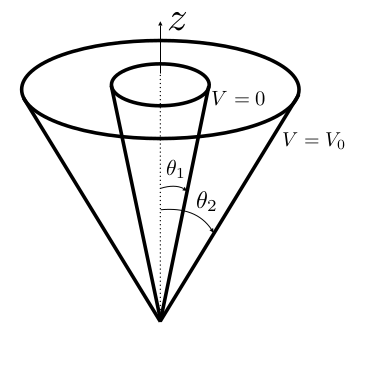
\includegraphics[width=0.4\textwidth]{figures/q8_fig1.png} % Substitua por seu nome de arquivo
\end{figure}

\textcolor{red}{\textbf{Solução:}}\\

% Solution Here

\subsection*{1. Equação de Laplace}

Em \colorbox{yellow!25}{coordenadas esféricas, supondo simetria axial e sem dependência radial} (isto é, \( V = V(\theta) \)), a equação de Laplace se reduz a:
\begin{equation}
\frac{1}{\sin \theta} \dv{\theta} \left(\textcolor{red}{ \sin \theta \dv{V}{\theta}} \right) = 0
\end{equation}

\subsection*{2. Solução Geral}

Integrando a equação acima:

\begin{align*}
\dv{\theta} \left( \textcolor{red}{ \sin \theta \dv{V}{\theta}} \right) &= 0 
\Rightarrow \sin \theta \dv{V}{\theta} = C_1 
\Rightarrow \dv{V}{\theta} = \frac{C_1}{\sin \theta} \\
V(\theta) &= C_1 \int \frac{1}{\sin \theta} \, d\theta + C_2 = C_1 \ln \left( \tan \frac{\theta}{2} \right) + C_2
\end{align*}

\subsection*{3. Condições de Contorno}

Aplicando as condições de contorno:

\begin{align*}
V(\theta_1) &= 0 \Rightarrow 0 = C_1 \ln \left( \tan \frac{\theta_1}{2} \right) + C_2 
\Rightarrow C_2 = -C_1 \ln \left( \tan \frac{\theta_1}{2} \right) \\
V(\theta_2) &= V_0 \Rightarrow V_0 = C_1 \left[ \ln \left( \tan \frac{\theta_2}{2} \right) - \ln \left( \tan \frac{\theta_1}{2} \right) \right] \\
&\Rightarrow C_1 = \frac{V_0}{\ln \left( \dfrac{\tan(\theta_2/2)}{\tan(\theta_1/2)} \right)}
\end{align*}

\subsection*{4. Potencial Elétrico}

Substituindo os coeficientes, obtemos o potencial elétrico:

\begin{equation}
\boxed{
V(\theta) = V_0 \cdot \frac{\ln \left( \dfrac{\tan(\theta/2)}{\tan(\theta_1/2)} \right)}{\ln \left( \dfrac{\tan(\theta_2/2)}{\tan(\theta_1/2)} \right)}
}
\end{equation}

\subsection*{5. Campo Elétrico}

O campo elétrico é dado por:

\begin{equation}
\vb{E} = -\grad V = -\frac{1}{r} \dv{V}{\theta} \, \hat{\bm{\theta}}
\end{equation}

Calculando a derivada:

\begin{align*}
\dv{V}{\theta} &= V_0 \cdot \frac{1}{\ln \left( \dfrac{\tan(\theta_2/2)}{\tan(\theta_1/2)} \right)} \cdot \dv{\theta} \left[ \ln \left( \tan \frac{\theta}{2} \right) \right] \\
&= V_0 \cdot \frac{1}{\ln \left( \dfrac{\tan(\theta_2/2)}{\tan(\theta_1/2)} \right)} \cdot \frac{1}{\sin \theta}
\end{align*}

Portanto:

\begin{equation}
\boxed{
\vb{E}(\theta) = -\frac{V_0}{r \ln \left( \dfrac{\tan(\theta_2/2)}{\tan(\theta_1/2)} \right)} \cdot \frac{1}{\sin \theta} \, \hat{\bm{\theta}}
}
\end{equation}
\end{flushleft}

\begin{flushleft}
\textbf{\textcolor{blue}{\Large Problema 9}}\\

Duas placas condutoras planas e infinitas são paralelas ao plano \( xy \). Uma está localizada
em \( z = 0 \) e mantida a potencial constante \( V_0 \). A outra, mantida a potencial 
constante \( V_d \), está em \( z = d \). A região entre elas contém uma densidade volumétrica 
de carga dada por:

\begin{equation}
\rho(z) = \rho_0 \left( \frac{z}{d} \right)^2
\end{equation}

Resolver a equação de Poisson para obter o potencial \( V(z) \) no intervalo \( 0 \leq z \leq d \), 
e determinar a densidade superficial de carga em cada uma das placas.

\textcolor{red}{\textbf{Solução:}}\\

% Solution Here

\section*{1. Equação de Poisson}

Em uma região com simetria unidimensional no eixo \( z \), a equação de Poisson é:

\begin{equation}
\frac{d^2 V}{dz^2} = -\frac{\rho(z)}{\varepsilon_0}
\end{equation}

Com a densidade dada por:

\begin{equation}
\rho(z) = \rho_0 \left( \frac{z}{d} \right)^2
\end{equation}

Temos:

\begin{equation}
\frac{d^2 V}{dz^2} = -\frac{\rho_0}{\varepsilon_0} \left( \frac{z}{d} \right)^2
\end{equation}

\section*{2. Integração da Equação}

Integrando uma vez:

\begin{equation}
\frac{dV}{dz} = -\frac{\rho_0}{\varepsilon_0 d^2} \int z^2 \, dz = -\frac{\rho_0}{\varepsilon_0 d^2} \cdot \frac{z^3}{3} + C_1
\end{equation}

Integrando novamente:

\begin{equation}
V(z) = -\frac{\rho_0}{\varepsilon_0 d^2} \cdot \frac{z^4}{12} + C_1 z + C_2
\end{equation}

\section*{3. Condições de Contorno}

As condições de contorno são:

\begin{equation}
V(0) = V_0 \quad \Rightarrow \quad C_2 = V_0
\end{equation}

\begin{equation}
V(d) = V_d \quad \Rightarrow \quad 
V_d = -\frac{\rho_0}{\varepsilon_0 d^2} \cdot \frac{d^4}{12} + C_1 d + V_0
\Rightarrow C_1 = \frac{V_d - V_0}{d} + \frac{\rho_0 d^2}{12 \varepsilon_0}
\end{equation}

\section*{4. Solução Final para o Potencial}

\begin{equation}
\boxed{
V(z) = -\frac{\rho_0 z^4}{12 \varepsilon_0 d^2} + \left( \frac{V_d - V_0}{d} + \frac{\rho_0 d^2}{12 \varepsilon_0} \right) z + V_0
}
\end{equation}

\section*{5. Campo Elétrico}

\begin{equation}
\vb{E}(z) = -\frac{dV}{dz} \, \hat{\vb{z}} = \left( \frac{\rho_0 z^3}{3 \varepsilon_0 d^2} - C_1 \right) \hat{\vb{z}}
\end{equation}

\section*{6. Densidade Superficial de Carga nas Placas}

Usamos:

\begin{equation}
\sigma = \varepsilon_0 E \quad \text{na interface com o condutor}
\end{equation}

\begin{itemize}
  \item Para \( z = 0 \):
  \begin{equation}
  E(0) = -\left( -C_1 \right) = C_1 \quad \Rightarrow \quad \boxed{\sigma_0 = \varepsilon_0 C_1}
  \end{equation}

  \item Para \( z = d \):
  \begin{equation}
  E(d) = \frac{\rho_0 d}{3 \varepsilon_0} - C_1 \quad \Rightarrow \quad 
  \boxed{\sigma_d = -\varepsilon_0 E(d) = \varepsilon_0 \left( C_1 - \frac{\rho_0 d}{3 \varepsilon_0} \right)}
  \end{equation}
\end{itemize}

\end{flushleft}

%%%%%%%% Bibliography 
% Os comandos para incluir as referências bibliográficas
%\printingbibliography

\end{document}
